\documentclass[conference]{IEEEtran}

\usepackage{inputenc}
%for referencing
%\usepackage[style=chicago,sorting=ynt]{biblatex}

\usepackage[sorting=none]{biblatex}
\addbibresource{references.bib}


%\usepackage{natbib}
%table related package
\usepackage{array}
\usepackage{tabu}
\usepackage{tabularx}
%for coloring table
\usepackage[table]{xcolor}
\usepackage{listings}
\usepackage{comment}
\usepackage{color}
%image related package
\usepackage{graphicx}
\graphicspath{ {./images/} }
%math related package
\usepackage{amsmath}
%\usepackage{amssymb}

%flooring and cailing
\usepackage{mathtools}
\DeclarePairedDelimiter\ceil{\lceil}{\rceil}
\DeclarePairedDelimiter\floor{\lfloor}{\rfloor}
%for algorithm
\usepackage{algorithm}
\usepackage{algorithmic}
%usepackage[options ]{algorithm2e}
%diagram related package 
\usepackage{tikz}
\usetikzlibrary{positioning,shapes,shadows,arrows}

%link coloring
\usepackage{hyperref}
\hypersetup{
    colorlinks,
    linkcolor={gray!50!black},
    citecolor={blue!60!black},
   urlcolor={blue!80!black}
}

%pagenumbering
%\pagenumbering{alpha}



\tikzstyle{line}=[draw,-latex']
\tikzstyle{elli}=[draw,ellipse,fill=blue!50,minimum height=10mm,node distance=5em]
\tikzstyle{block}=[draw,rectangle,fill=blue!50,text centered,minimum height=10mm,node distance=5em]

\begin{document}
\title{Huffman coding in data compression}
\author{
\IEEEauthorblockN{Md. Ismail\hspace{5em} Nabonitta Biwsas\\Roll No:1503094\hspace{3em}Roll No:1503095}

\IEEEauthorblockA{Department of Computer Science and Engineering \\
Rajshahi University of Engineering and Technology}
}

\date{}
\maketitle


\begin{abstract}
Huffman coding is a greedy lossless data compression algorithm. This technique  use   variable length encoding. Encoding also satisfies prefix rule of encoding. In this paper we will show mathematically how Huffman coding  compress data such as text file. We also compare Huffman data compression technique with ASCII system.
    
\end{abstract}
\section{Introduction}
\label{sec:intro}
\subsection{\textbf{Data compression:}}
Generally data compression is modifying the data in such a way that resulting modified data take less space than input data.It includes a stream of symbols and transforming them into codes\cite{nelson1995data}.
Data-compression techniques can be divided into two major families.\cite{nelson1995data}


 \begin{enumerate}
 \label{list:into1}
 \item Lossy data compression
  \item Lossless data compression
  
\end{enumerate}

\subsection{\textbf{Lossy and lossless data compression:}}
Difference between lossy data compression and lossless data compression is given bellow:

\begin{table}[h!]
   
        
    
%{\rowcolors{1}{green!80!yellow!50}{green!70!yellow!40}
\caption{Difference between lossy data compression and losless data compression} 
  \label{table:lossy}
  \begin{tabu} to 0.5 \textwidth  {|X[l]|X[l]|}
  \hline
      Lossy data compression & 
       Lossless data compression\\
       \hline
       Additional and unnecessary
       data is discards from input data\cite{nelson1995data}
       & No information is discarded\cite{nelson1995data}\\
       \hline
       Used where where perfect reproduction is not required\cite{ng1997lossless} & Used where perfect reproduction is required\cite{ng1997lossless}\\
       \hline
       Applied in 3D data transferring, multimedia file compression such as JPEG file,MP3 file,MP4 file, digitized voice recognition\cite{nelson1995data,ng1997lossless} & Data storing in database ,spreadsheets,word processing files. ,text file compression, compress medical images\cite{nelson1995data,ng1997lossless}\\
       \hline
      
  \end{tabu}
 % }
  
    
\end{table}
In ASCII (American Standard Code for Information Interchange)  each character is represented by eight bits of 0s and 1s binary string.But in Huffman encoding technique each character represent by different length of binary string in such a way that more common symbols are represented with fewer bits.\cite{han2015deep}
Generally there are two types of encoding system.
\begin{enumerate}
%\caption{Type of encoding system}
\label{list:into2}
%\color{blue} %to use color
  \item Fixed length encoding 
  \item Variable length encoding
\end{enumerate}
Fixed length means that length of the code for any character is fixed where variable length encoding means that length of the code is variable.Variable length encoding is mere better than fixed length encoding.\cite{cormen2009introduction}

\subsection{\textbf{Prefix rule:}}
In Huffman data compression technique bit string that represent a symbol or character is not prefix of the bit string which represent others symbol.\cite{cormen2009introduction}Which is known as prefix rule.As a result  ambiguity is removed during decoding time. \\
\textbf{Example:} If we find the set of bit string after decoding \[ \left \{t=0,u=11,e=100,r=101 \right\} \] is a prefix code.Now by encoding the bit string $"$0100101101$"$ we find only $"$terr$"$.This can be illustrated in the figure.

\begin{figure}[h]
\centering

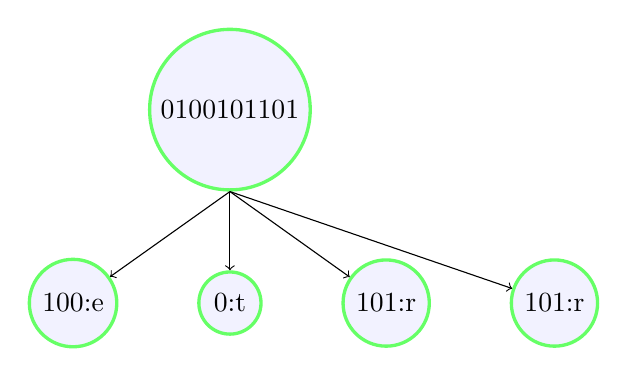
\begin{tikzpicture}[roundnode/.style={circle, draw=green!60, fill=blue!5, very thick, minimum size=7mm},
squarednode/.style={rectangle, draw=red!60, fill=red!5, very thick, minimum size=5mm},
]
%node
\node[roundnode]      (main)                              {0100101101};

\node[roundnode]      (bellow1)                          [below=of main]    {0:t};
\node[roundnode]      (bellow2)                          [left=of bellow1]    {100:e};
\node[roundnode]      (bellow3)                        [right=of bellow1]      {101:r};
\node[roundnode]      (bellow4)                        [right=of bellow3]      {101:r};

\draw[->](main.south)--(bellow1);
\draw[->](main.south)--(bellow2);
\draw[->](main.south)--(bellow3);
\draw[->](main.south)--(bellow4);


\end{tikzpicture}

\caption{Tree representation of prefix rule }
    
\end{figure}



But the bit string set     \[ \left \{x=0,y=1,z=11\right\}\] is not a prefix code because the string "111" can be represented as "yyy" or "yz" or "zy".This can be illustrated in the figure.
\begin{figure}
\centering

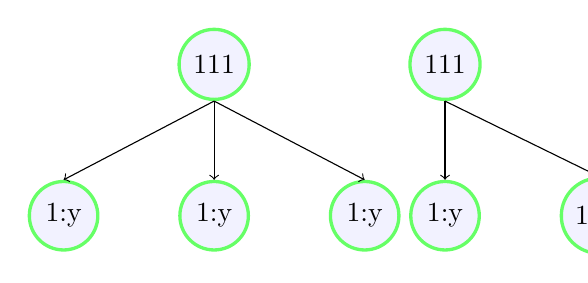
\begin{tikzpicture}[roundnode/.style={circle, draw=green!60, fill=blue!5, very thick, minimum size=7mm},
squarednode/.style={rectangle, draw=red!60, fill=red!5, very thick, minimum size=5mm},
]
%node
\node[roundnode]      (main1)                              {111};

\node[roundnode]      (lower1)                          [below=of main1]    {1:y};
\node[roundnode]      (lower2)                          [left=of lower1]    {1:y};
\node[roundnode]      (lower3)                        [right=of lower1]      {1:y};


%line
\draw[->] (main1.south) -- (lower1.north);
\draw[->] (main1.south) -- (lower2.north);
\draw[->] (main1.south) -- (lower3.north);

\hspace{1cm}
%node
\node[roundnode]      (main2)                         [right=of main1 ]      {111};

\node[roundnode]      (lower4)                          [below=of main2]    {1:y};
\node[roundnode]      (lower5)                          [right=of lower4]    {11:z};
%line

\draw[->] (main2.south) -- (lower4.north);
\draw[->] (main2.south) -- (lower5.north);

\end{tikzpicture}

\caption{Tree representation not a prefix rule }
    
\end{figure}



\par We organized our paper as follow. In section\ref{sec:meth} Huffman algorithm will be discussed.Experimental result with some mathematical calculation will be demonstrated in
section \ref{sec:exp}. In this section we also compare Huffman coding with ASCII coding ,Arithmetic coding.Finally in section \ref{sec:con} advantages and disadvantages of Huffman coding will be mentioned.    

\section{Background}
When transferring a message of data or text ,if transmission time for each symbol is same then  transmission time of message is directly proportional to length of message code.\cite{huffman1952method}.For this reason transferring message use ASCII and EBCDIC  code take a long time also a huge amount of empty memory whereas variable length code need $\ceil*{log_2n}$ bit per letter\cite{vitter1987design}.David A. Huffman publish a paper where he propose a coding system based on the probability of character in message. 


\section{Methodology}
\label{sec:meth}
Generally there are two steps of Huffman coding.They are:
\begin{itemize}
  \item Constructing a Huffman tree from input data of character
  \item Traversing the Huffman tree and determining the code of the character
\end{itemize}
\subsection{\textbf{Constructing a Huffman tree:}}

Huffman tree can be built from the frequency of the character.Which is known as statistical modeling.\cite{nelson1995data}Following are the process\cite{sharma2010compression} of constructing a Huffman tree by using min heap:
\renewcommand{\labelenumi}{\roman{enumi}}
%for changing  numbering style of list



\begin{enumerate}
\label{list:e1}
\item Make all the character leaf node of tree.
\item Push all the character  into min priority queue i.e., characters are in ascending order of their frequency.
\item Pop first two element of priority queue and push their (first two element) sum as the top of priority queue.
\item Repeat step 3 till priority queue contain more than one  node.
\item Now tree is generated and remaining  node  is the root node of the Huffman tree.
\end{enumerate}
\vspace{.5cm}
Huffman tree are built from the bottom up\cite{nelson1995data}.
Algorithm~\ref{alg:alg1} is the Huffman tree construction algorithm:\cite{cormen2009introduction}
%Huffman algorithm
\begin{algorithm}[H]
\begin{algorithmic}
\STATE $n\gets$ no of character
\FOR{$i=0$ to $n-1$}
 \STATE $min heap$ $.$ $push$ $($character,frequency$)$
 \STATE $i\gets i-1$
 \ENDFOR
 \WHILE{$min heap$ $.$$size()$$>1$}
 \STATE create a new node N
 \STATE $N.left\gets $ top of min heap
 \STATE pop min heap
 \STATE $N.right\gets$ top of min heap
  \STATE pop min heap
  \STATE $N.top\gets$ $ N.left+N.right$
  \STATE $min heap$ $.push(top)$
  \ENDWHILE
 \RETURN min heap
\end{algorithmic}
\caption{Huffman(no of character)}
\label{alg:alg1}
\end{algorithm}

%\subsection{\textbf{Traversing a Huffman tree:}}
To determine the code of character we traverse the Huffman tree by using a recursive function. Algorithm~\ref{alg:alg2} is the algorithm of traversing Huffman tree.

\begin{algorithm}[H]
\begin{algorithmic}
\IF{root is null}
\RETURN 
\ENDIF
\IF{symbol of root is not null}
\STATE print code
\ENDIF

\STATE Traverse(left child of root,$code+0$)
\STATE Traverse(right child of root,$code+1$)



\end{algorithmic}
\caption{Traverse(root node,code)}
\label{alg:alg2}
\end{algorithm}


 


%subsection{\textbf{Decoding code:}}
\par Decoding code is very easy.We use STL to decode the text file. Following algorithm \ref{alg:alg3} is the pseudo code for decoding.
\begin{algorithm}[H]
\begin{algorithmic}
\STATE $s\gets$ input encoding string
\STATE $n\gets$ no of individual character
\STATE declare map$<char,string>$code
\FOR{$i=0$ to $n-1$}

\STATE code$.$insert$(make\_pair(symbol,code))$
\ENDFOR
\STATE declare string $f$ as NULL to store decode string 
\STATE declare  temporary string $x$ as NULL 
\FOR{$i=0$ to length of $s$}
\STATE $x\gets x+s[i]$ 
\STATE declare an iterator $it=code.begin()$
\WHILE{$it!=code.end()$}
\IF{$it->second==x$}
\STATE $f=f+it->first$
\STATE break
\ENDIF
\STATE $it\gets it+1$
\ENDWHILE
  
\ENDFOR
\STATE print $f$


\end{algorithmic}
\caption{Pseudo code of decoding}
\label{alg:alg3}
\end{algorithm}

\par \textbf{Complexity analysis:}For n nodes pop operation into while loop of \ref{alg:alg1} will execute  (n-1) times.Each of loop take complexity of O(logn).
So complexity of Huffman tree constructing algorithm is O(nlogn).
\section{Experiment}
\label{sec:exp}
\par \textbf{Example:}
\label{exa:tree}
A file containing frequencies shown at  table~\ref{table:exam}.Determine the Huffman code of each symbol.
\begin{table}[h]
\caption{Symbol with frequencies}
\label{table:exam}
  \begin{tabu} to 0.5\textwidth { |X[c] | X[c]| }
 \hline
 Symbol & Frequencies  \\
 \hline
 a & 15\\
 \hline
 e & 3\\
 \hline
 i & 4\\
 \hline
 o & 10\\
 \hline
 u & 1\\
 \hline
 
\end{tabu} 
 
\end{table}

\par \textbf{Solution:}Now construct Huffman tree step by step.Figure \ref{fig:my_label1} to figure \ref{fig:my_label5} illustrate different steps of above example. \\
step1:\\
\begin{figure}[H]
\centering
    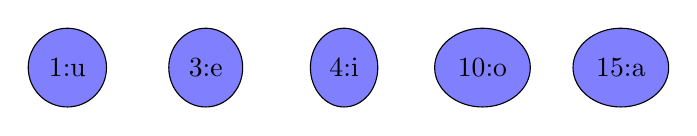
\begin{tikzpicture}
%node
\node[elli](leaf1){1:u};
\node[elli,right of=leaf1](leaf2){3:e};
\node[elli,right of=leaf2](leaf3){4:i};
\node[elli,right of=leaf3](leaf4){10:o};
\node[elli,right of=leaf4](leaf5){15:a};


%arrows
\end{tikzpicture}
    \caption{Huffman tree after first pass}
    \label{fig:my_label1}
\end{figure}
Step2:\\
\begin{figure}[H]
\centering
    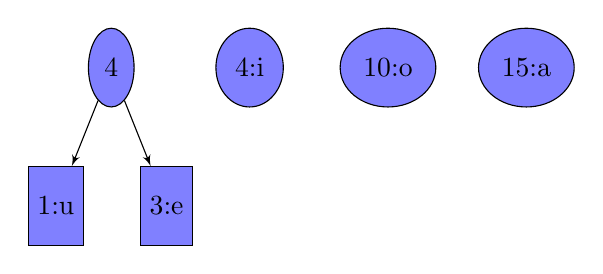
\begin{tikzpicture}
%node
\node[elli](root){4};
\node[block,below of=root,xshift=-2em](left){1:u};
\node[block,below of=root,xshift=+2em](right){3:e};
\node[elli,right of=root](leaf1){4:i};
\node[elli,right of=leaf1](leaf2){10:o};
\node[elli,right of=leaf2](leaf3){15:a};
%arrows
\path[line](root)--(left);
\path[line](root)--(right);
\end{tikzpicture}
    \caption{Huffman tree after second pass}
    \label{fig:my_label2}
\end{figure}
step3:\\
\begin{figure}[H]
\centering
    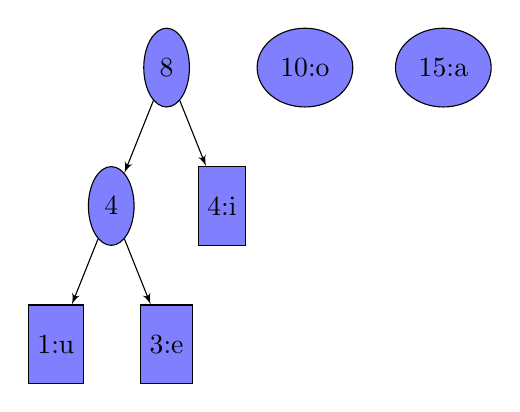
\begin{tikzpicture}
\node[elli](root){8};
\node[elli,below of=root,xshift=-2em](left){4};
\node[block,below of=root,xshift=+2em](right){4:i};
\node[block,below of=left,xshift=-2em](left1){1:u};
\node[block,below of=left,xshift=+2em](right1){3:e};

\node[elli,right of=root](leaf1){10:o};
\node[elli,right of=leaf1](leaf2){15:a};


%arrows
\path[line](root)--(left);
\path[line](root)--(right);
\path[line](left)--(left1);
\path[line](left)--(right1);
\end{tikzpicture}
    \caption{Huffman tree after third pass}
    \label{fig:my_label3}
\end{figure}


Step4:\\
\begin{figure}[H]
\centering
    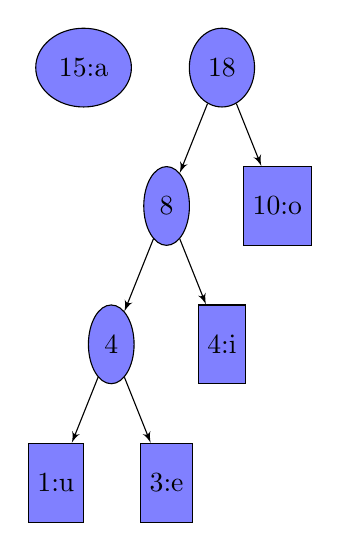
\begin{tikzpicture}
\node[elli](root){18};
\node[elli,below of=root,xshift=-2em](left){8};
\node[block,below of=root,xshift=+2em](right){10:o};
\node[elli,below of=left,xshift=-2em](left1){4};
\node[block,below of=left,xshift=+2em](right1){4:i};
\node[block,below of=left1,xshift=+2em](right2){3:e};
\node[block,below of=left1,xshift=-2em](left2){1:u};

\node[elli,left of=root](leaf1){15:a};


%arrows
\path[line](root)--(left);
\path[line](root)--(right);
\path[line](left)--(left1);
\path[line](left)--(right1);
\path[line](left1)--(left2);
\path[line](left1)--(right2);
\end{tikzpicture}
    \caption{Huffman tree after forth pass}
    \label{fig:my_label4}
\end{figure}
    

Step5: In this step Huffman tree is created.Bit '0' represent the left child and bit '1' represent right child.\cite{sharma2010compression}

\begin{figure}[H]
\centering
    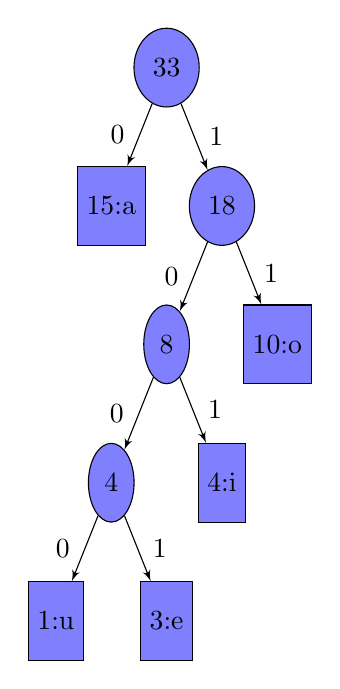
\begin{tikzpicture}
\node[elli](root){33};

\node[block,below of=root,xshift=-2em](left){15:a};
\node[elli,below of=root,xshift=+2em](right){18};

\node[elli,below of=right,xshift=-2em](left1){8};
\node[block,below of=right,xshift=+2em](right1){10:o};

\node[block,below of=left1,xshift=+2em](right2){4:i};
\node[elli,below of=left1,xshift=-2em](left2){4};

\node[block,below of=left2,xshift=-2em](left3){1:u};
\node[block,below of=left2,xshift=+2em](right3){3:e};




%arrows
\path[line](root)--node[xshift=-.8em]{0}(left);
\path[line](root)--node[xshift=+.8em]{1}(right);
\path[line](right)--node[xshift=-.8em]{0}(left1);
\path[line](right)--node[xshift=+.8em]{1}(right1);
\path[line](left1)--node[xshift=-.8em]{0}(left2);
\path[line](left1)--node[xshift=+.8em]{1}(right2);
\path[line](left2)--node[xshift=-.8em]{0}(left3);
\path[line](left2)--node[xshift=+.8em]{1}(right3);
\end{tikzpicture}
    \caption{Final Huffman tree }
    \label{fig:my_label5}
\end{figure}
\par To determine the Huffman code of each symbol traverse Huffman tree starting from the root node to the every leaf node.Code of each symbol is tabulated at table \ref{table:code}.
\begin{table}[h]
\caption{Symbol with their code}
\label{table:code}
  \begin{tabu} to .5\textwidth { |X[c] | X[c]| X[c]| X[c]|X[c]|}
 \hline
 Symbol & Huffman Code &Length of Huffman code & ASCII code & Length of ASCII code\\
 \hline
 a & 0 & 1 & 01100001 & 8\\
 \hline
 o & 11 & 2 & 01101111 & 8\\
 \hline
 
 i & 101 & 3 & 01101001 & 8\\
 \hline
 
 e & 1001 & 4 & 01100101 & 8\\
 
 \hline
 u & 1000 & 4 & 01110101 & 8\\
 \hline
 
\end{tabu} 
 
\end{table}

From table \ref{table:code} it is proved that the length of code is variable whereas length of ASCII code is fixed.Average length of ASCII code is 8.Average length of Huffman code is determined by using formula \ref{equ:1}\cite{cormen2009introduction} and the number of bits in encoded message is determined by formula \ref{equ:2}\cite{cormen2009introduction}.Entropy of Huffman can be determined by using formula \ref{equ:3}.\cite{howard1994arithmetic}

\begin{equation}
\label{equ:1}
    average\hspace{.5em} length\hspace{.5em} of\hspace{.5em} code  = \frac{\sum (frequency_i \hspace{.5em} \times \hspace{.5em} code\hspace{.5em} length_i)}{\sum frequency_i}
\end{equation}

\textit{number of bits in encoded message,}
\begin{equation}
\label{equ:2}
    =(\sum number\hspace{.5em}of\hspace{.5em}character\hspace{.5em} \times \hspace{.5em} average\hspace{.5em}length\hspace{.5em}of\hspace{.5em}bit)
\end{equation}

\begin{equation}
\label{equ:3}
    H(x)=\sum_{k=1}^{k=n}-p_k log_2p_k
\end{equation}


For Huffman code of table \ref{table:code} average length of code ,\\

 $$ L = \frac{(15*1)+(10*2)+(4*3)+(3*4)+
(1*4)}{(15+10+4+3+1)}$$
$$=1.909 $$
As Huffman coding use integral number of bit of code word it is 2.\cite{nelson1995data}
% $$\approx2$$
Hence percentage of compression of data by using Huffman coding, $$=\frac{8-2}{8}\times100$$

$$=75$$


\begin{table}[h]
\caption{Probability table of table\ref{table:code}}
\label{table:pro}
  \begin{tabu} to .5\textwidth { |X[c] | X[c]| X[c]| X[c]|X[c]|}
 \hline
 Symbol & Length of Huffman code & $$ p_k $$ & $$log_2p_k$$ & $$p_klog_2p_k$$\\
 \hline
 a & 1 & 0.4545 & -1.1376 & 0.51703\\
 \hline
 o & 2 & 0.0909 & -1.0414 & 0.0946\\
 \hline
 
 i & 3 & 0.1212 & -0.9164 & 0.11106\\
 \hline
 
 e & 4 & 0.3030 & -0.51855 & 0.1572\\
 
 \hline
 u & 4 & 0.030030 & -1.5122 & 0.04541\\
 \hline
  & & & & $$\sum=.9253$$\\
  \hline
 
\end{tabu} 
 
\end{table}

Now by using data from table \ref{table:pro}  and formula 
\ref{equ:3}
find the entropy ,
$$H(x)=0.9253$$
Hence the percentage of  efficiency of the Huffman coding data compression,$$\eta =\frac{H(x)}{L}$$
$$=\frac{0.9253}{1.909}\times100\\
=48.45$$\\

\subsection{\textbf{Result analysis:}}
In our calculation we show that efficiency  is almost 50 percent and it can compress 75 percent than normal ASCII coding.In generally it varies from 20 percent to 90 percent which is depend on the property of data being  compressed.\cite{cormen2009introduction} 
\section{Conclusion}
Main advantages of Huffman coding is it is easy to implement.But it depends on statistical model of data.If there is a wrong in the statistical data it does not give correct compression.Although Huffman coding is better than ASCII coding , it has some demerits. It uses integer number of code length.So it is does not give good data compression.Arithmetic coding data compression technique can remove this.
\label{sec:con}
\printbibliography
\end{document}
  


